\begin{table}[H]\centering\small
\begin{tabular}{@{}lrrrr@{}}\toprule
Frozen policy & Net collections & Complete cost & Profit & Available cash \\ \midrule
U & 1,431.72 & 469.11 & 962.61 & 1,938.61 \\
E & 1,431.72 & 499.11 & 932.61 & 1,908.61 \\
E+ equipped & 1,431.72 & 521.21 & 910.51 & 1,886.51 \\
Private option & 1,430.08 & 511.06 & 919.01 & 1,895.02 \\
Shared option & 1,430.08 & 511.09 & 918.99 & 1,894.99 \\
Library option & 1,430.08 & 511.09 & 918.99 & 1,894.99 \\
\bottomrule\end{tabular}
\caption{Original limited-controller reference scenario: mean USD per 30 operating days plus 14 settlement days, 128 worlds per policy. Initial capital is USD1,000; the selected reserve is USD24. All figures are modeled, including failed work and prototypes.}
\end{table}
Every policy selected a 0.5 price/reference ratio and three days of reserve from the declared development grid. The component price is therefore modeled at \$35 against an assumed \$70 human-service reference. The observed acceptance counts provide no quality increment, and equal-quality uncertainty is coupled. The original E--U difference is exactly the assumed \$30 method setup cost, not an estimated market value of expert prompting. Equipped E+ adds assumed packaging, invocation and maintenance expense. The original shared-option policy loses \$13.62 relative to E, with conditional Monte Carlo 95\% interval [\$-15.10, \$-12.15]. Its one reference-profile admission is a modeled assessor error. Graph and identical-content library trajectories match exactly. No Gym campaign is selected in the tested primary or stress runs. This tests optional restraint; it does not empirically test a trained specialist.

The simulated four-component pack is an illustrative bundle, not the separately executed C5 campaign auditor. These enterprise results neither price nor validate C5. The initial controller selects pricing and reserves but evaluates an assessment option without a separate learned HOLD choice; the additive value-controller experiment below corrects that decision-menu limitation prospectively.
\begin{table}[H]\centering\small
\begin{tabular}{@{}lrrr@{}}\toprule
U scenario & Mean profit & 10th percentile & Loss worlds \\ \midrule
Thin demand & 80.63 & -115.08 & 51/128 \\
Lower-price human & 73.88 & -70.46 & 42/128 \\
5 residual minutes & 657.26 & 197.97 & 1/64 \\
15 residual minutes & 40.43 & -179.44 & 16/64 \\
10x model charge & 21.32 & -202.44 & 19/64 \\
\bottomrule\end{tabular}
\caption{Conditional USD scenarios with the same frozen policy. Lower demand, cheaper alternatives and residual obligations can make the modeled service unprofitable in many worlds.}
\end{table}
\begin{figure}[H]\centering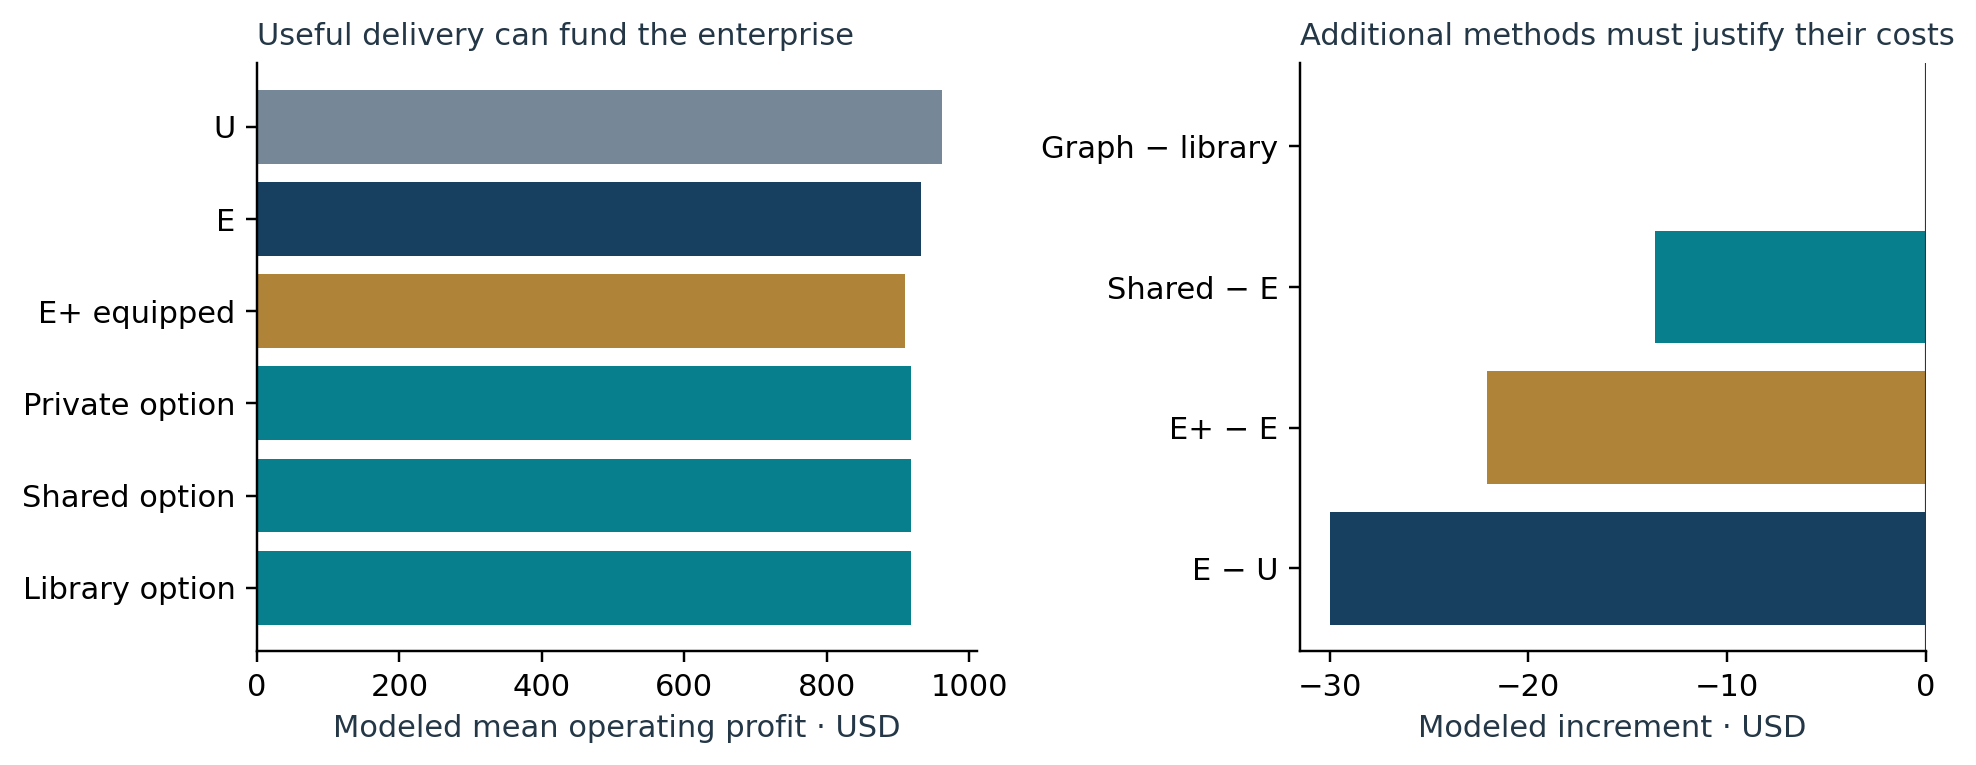
\includegraphics[width=0.95\linewidth]{figures/economics_original.png}\caption{These increments follow from assumptions about costs and no accepted-output gain; they are not observed monetary Alpha. The optional-controller improvement is reported separately.}\end{figure}
